\ESKDstyle{title}
\thispagestyle{plain}
\pagestyle{plain}
\hspace{0pt}

Таблицы в базе данных:
\begin{itemize}
    \item \textbf{СП\_ЕдХран} - см. рис.~\ref{fig:CP_EdXran}
    \item \textbf{СП\_Произв} - см. рис.~\ref{fig:CP_Proizv}
    \item \textbf{СП\_МоиОрг} - см. рис.~\ref{fig:CP_MoiOrg}
    \item \textbf{СП\_ДолжСотр} - см. рис.~\ref{fig:CP_DoljSotr}
    \item \textbf{СП\_Сотр} - см. рис.~\ref{fig:CP_Sotr}
    \item \textbf{СП\_МестаХран} - см. рис.~\ref{fig:CP_MestaXran}
    \item \textbf{СП\_Номенкл} - см. рис.~\ref{fig:CP_Nomencl}
    \item \textbf{КомИнвент} - см. рис.~\ref{fig:CP_KomInvent}
    \item \textbf{ТабличнаяЧасть\_СоставКомис} - см. рис.~\ref{fig:TablichnajaChast_SostavKomissii}
    \item \textbf{ОП\_ИнвенОпис} - см. рис.~\ref{fig:OP_InvenOpis}
    \item \textbf{ОП\_ПриказСоздКомИнвент} - см. рис.~\ref{fig:OP_PrikazSozdKomInvent}
    \item \textbf{ТабличнаяЧасть\_Номенкл} - см. рис.~\ref{fig:TablichnajaChast_Nomencl}
\end{itemize}

\lstinputlisting[language=sql]
    {src/create.sql}

\begin{figure}[!h]
    \centering
    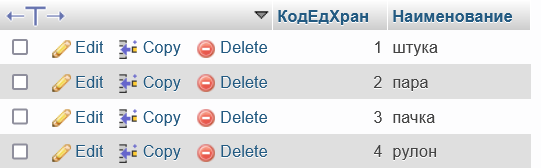
\includegraphics[width=12cm]
        {_assets/СП_ЕдХран.png}
    \caption{Таблица справочного документа <<Единицы хранения>> в БД}
    \label{fig:CP_EdXran}
\end{figure}

\begin{figure}[!h]
    \centering
    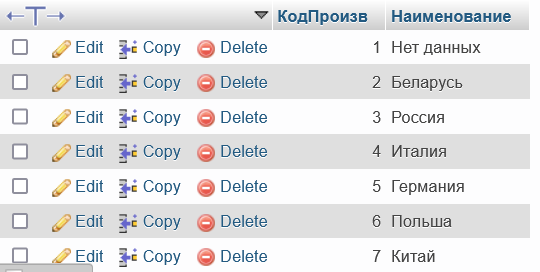
\includegraphics[width=12cm]
        {_assets/СП_Произв.png}
    \caption{Таблица справочного документа <<Производители>> в БД}
    \label{fig:CP_Proizv}
\end{figure}

\begin{figure}[!h]
    \centering
    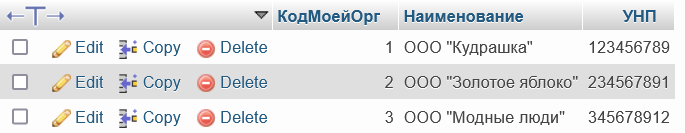
\includegraphics[width=12cm]
        {_assets/СП_МоиОрг.png}
    \caption{Таблица справочного документа <<Мои организации>> в БД}
    \label{fig:CP_MoiOrg}
\end{figure}

\begin{figure}[!h]
    \centering
    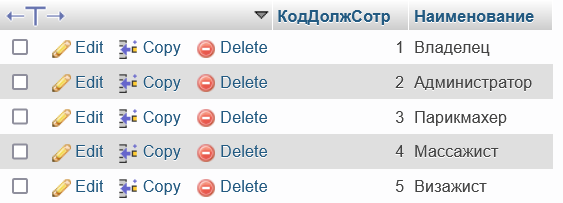
\includegraphics[width=12cm]
        {_assets/СП_ДолжСотр.png}
    \caption{Таблица справочного документа <<Должности сотрудника>> в БД}
    \label{fig:CP_DoljSotr}
\end{figure}

\begin{figure}[!h]
    \centering
    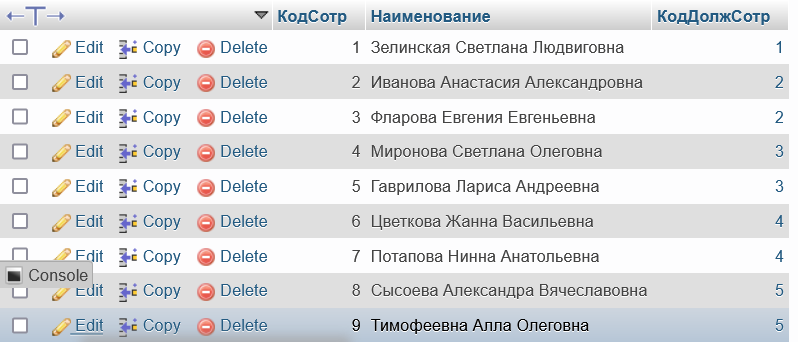
\includegraphics[width=12cm]
        {_assets/СП_Сотр.png}
    \caption{Таблица справочного документа <<Сотрудники>> в БД}
    \label{fig:CP_Sotr}
\end{figure}

\begin{figure}[!h]
    \centering
    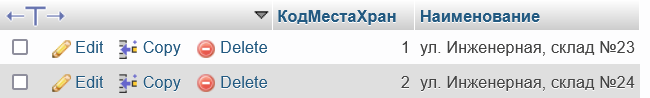
\includegraphics[width=12cm]
        {_assets/СП_МестаХран.png}
    \caption{Таблица справочного документа <<Места хранения>> в БД}
    \label{fig:CP_MestaXran}
\end{figure}

\begin{figure}[!h]
    \centering
    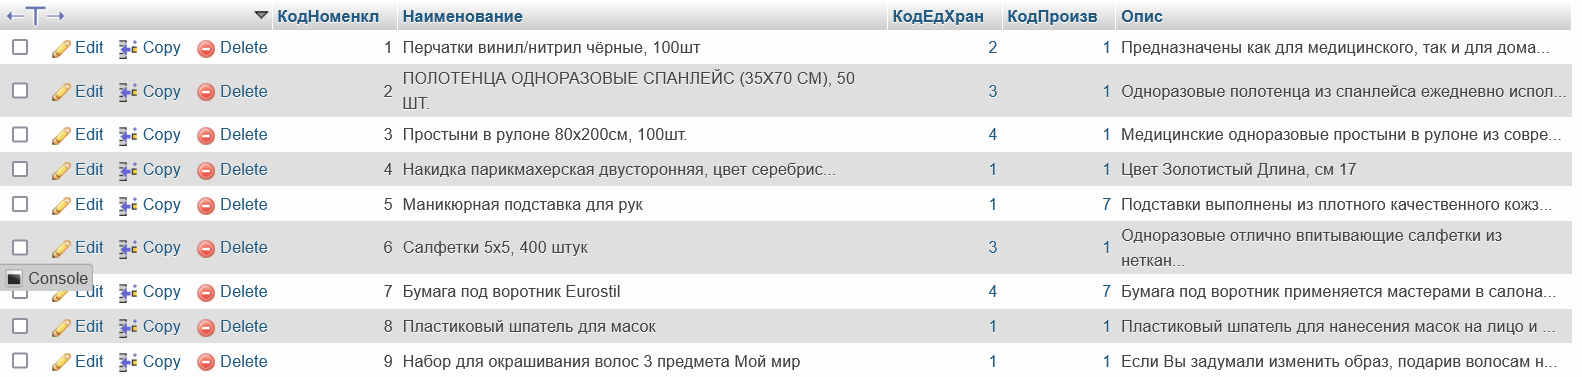
\includegraphics[width=18cm]
        {_assets/СП_Номенкл.png}
    \caption{Таблица справочного документа <<Номенклатура>> в БД}
    \label{fig:CP_Nomencl}
\end{figure}

\begin{figure}[!h]
    \centering
    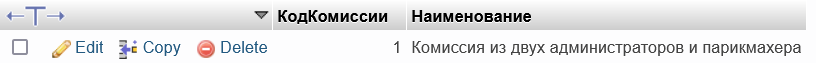
\includegraphics[width=12cm]
        {_assets/КомИнвент.png}
    \caption{Таблица <<Коммисия инвентаризационная>> в БД}
    \label{fig:CP_KomInvent}
\end{figure}

\begin{figure}[!h]
    \centering
    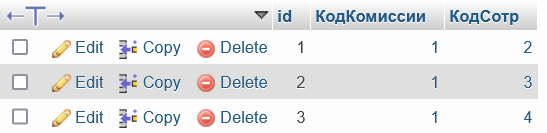
\includegraphics[width=12cm]
        {_assets/ТабличнаяЧасть_СоставКомис.png}
    \caption{Таблица <<Табличная часть - Состав комиcсии>> в БД}
    \label{fig:TablichnajaChast_SostavKomissii}
\end{figure}

\begin{figure}[!h]
    \centering
    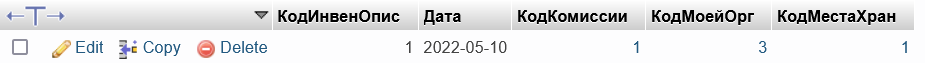
\includegraphics[width=12cm]
        {_assets/ОП_ИнвенОпис.png}
    \caption{Таблица оперативного документа <<Инвентаризационная опись>> в БД}
    \label{fig:OP_InvenOpis}
\end{figure}

\begin{figure}[!h]
    \centering
    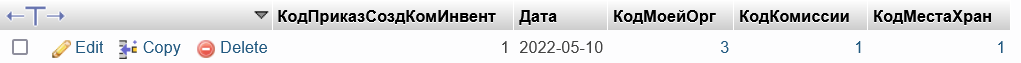
\includegraphics[width=12cm]
        {_assets/ОП_ПриказСоздКомИнвент.png}
    \caption{Таблица оперативного документа <<Приказ о создании комиссиии инвентаризационной>> в БД}
    \label{fig:OP_PrikazSozdKomInvent}
\end{figure}

\begin{figure}[!h]
    \centering
    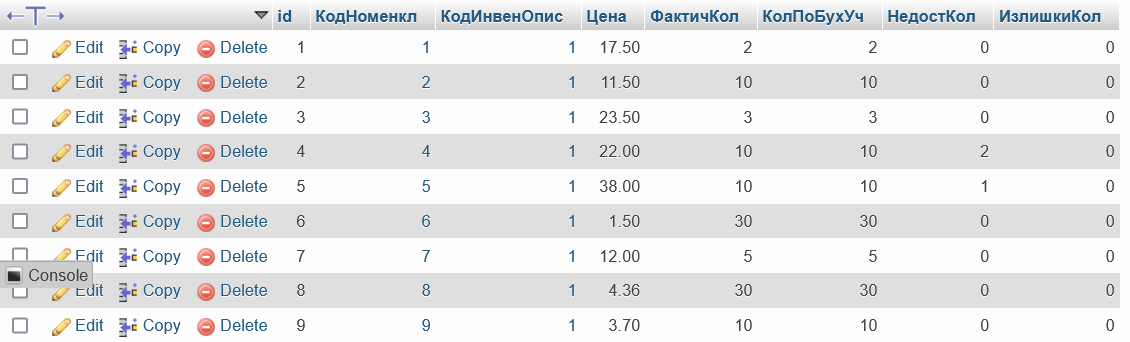
\includegraphics[width=18cm]
        {_assets/ТабличнаяЧасть_Номенкл.png}
    \caption{Таблица <<Табличная часть - Номенклатура>> в БД}
    \label{fig:TablichnajaChast_Nomencl}
\end{figure}
